\section{Photometric redshift estimation}

For our symbolic regression we rely on PySR\cite{pysr}. It uses genetic programming to find a symbolic expression for a numerically defined function in terms of pre-defined variables. The population consists of symbolic expressions, visualized as a tree and consisting of nodes with an operator function or an operand. We use the operators for addition, subtraction, multiplication. The tree population evolves when new individuals are created and old ones are discarded. To breed the next generation, several mutation operators can be applied, for instance exchanging, adding or deleting nodes of the parent tree. The hyperparameter populations = 30 defines the number of populations and is per default set to the number of processors used (procs). The number of individuals per populations is given by npop = 1000. As the figure of merit for the PySR algorithm we take the mean squared error between the data points $t_{i}(x, z|\theta)$ and the functional description $g_i$
\begin{equation}
	MSE = \frac{1}{n} \sum_{i=1}^{n} \left( g_{i}\left(x\right) - t_{i}(x, z|\theta) \right)
\end{equation}
and balance it with the function’s complexity, defined as
\begin{equation}
	complexity = \# nodes
\end{equation}
For the PySR score value, not to be confused with the statistics version of the optimal observable defined in, the parameter parsimony balances the two conditions,
\begin{equation}
	score = \frac{MSE}{baseline} + parsimony \times complexity
\end{equation}
The normalization factor baseline is the MSE between the data and the constant unit function. The hyperparameter $maxsize$ restricts the complexity to a maximum value. We adjust this value depending on the difficulty of the regression task taking 50 as a starting point and increase (decrease) it if the required complexity is larger (smaller). Additionally we can restrict the complexity of specific operators to obtain a more readable result. We set the maximal complexity of square to 5 and cube to 3. Note that in some instances we choose to not extract the score, but the score scaled by a constant, to improve the numerics with an order-one function. Simulated annealing allows us to search for a global optimum in a high-dimensional space while preventing the algorithm from being stuck in a local optimum. A mutation is accepted with the probability
\begin{equation}
	p = exp\left( - \frac{score_{new} - score_{old}}{alpha\times T} \right)
\end{equation}
The parameter T is referred to as temperature. It linearly decreases with each cycle or generation, starting with 1 in the first cycle and 0 in the last. The hyperparameter ncyclesperiterations = 200 sets the amount of cycles. We choose alpha = 1. If the new function describes the data better than the reference tree, $score_{new}$ $score_{old}$, the exponent has a positive sign and the new function is accepted. If the new sore is larger than the old score, the acceptance of the new function is given by p and hence exponentially suppressed. We use this default PySR form for our simple example and discuss a bettersuited form for our application in Sec. 3. The hyperparameter niterations = 300 defines the number of iterations of a full simulated annealing process. After each iteration the best formulas are compared to the hall of fame (HoF). For each complexity the best equation is chosen and saved in the output file. An equation of higher complexity is only added if its MSE is smaller than for previous formulas. Equations from different populations or the hall of fame can migrate to other populations. This process is affected by the parameters fractionReplaced = 0.5 and fractionReplacedHof = 0.2.
\begin{figure}
	\centering
	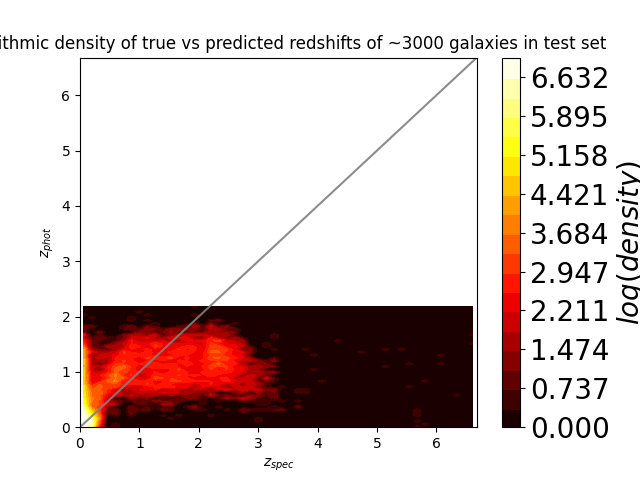
\includegraphics[width=\textwidth]{density_plot.png}
	\caption{Photometric redshift prediction and errorbars for a representative subsample of 300 galaxies. The errorbars are due to errors in the photometric data and so depend on the particular model chosen for $z_{phot}$}
	\label{fig:density_plot}
\end{figure}
\begin{figure}
	\centering
	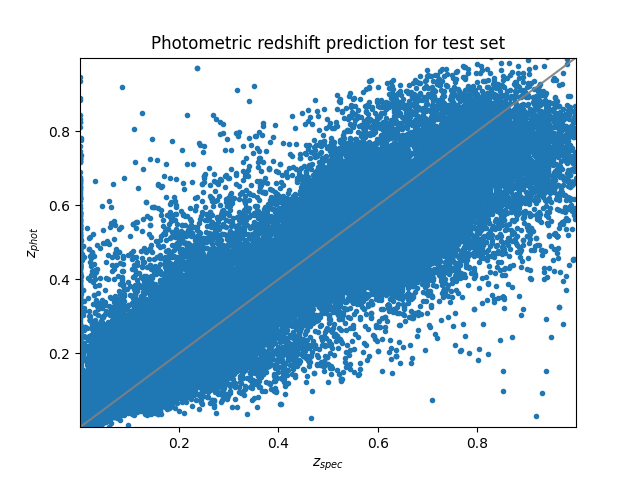
\includegraphics[width=\textwidth]{predictions.png}
	\caption{Predictions for test data}
	\label{fig:predictions}
\end{figure}
\begin{figure}
	\centering
	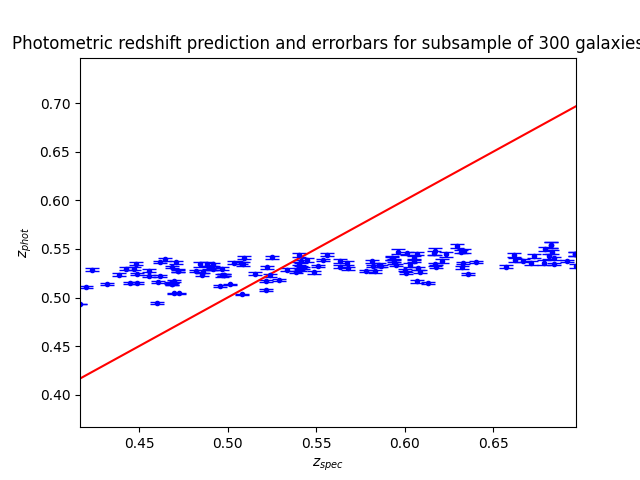
\includegraphics[width=\textwidth]{predictions_with_error.png}
	\caption{Photometric redshift prediction and errorbars for a representative subsample of 300 galaxies. The errorbars are due to errors in the photometric data and so depend on the particular model chosen for $z_{phot}$}
	\label{fig:predictions_with_error}
\end{figure}